\newcommand{\inputs}{5}
\newcommand{\hiddens}{3}
\newcommand{\outputs}{5}

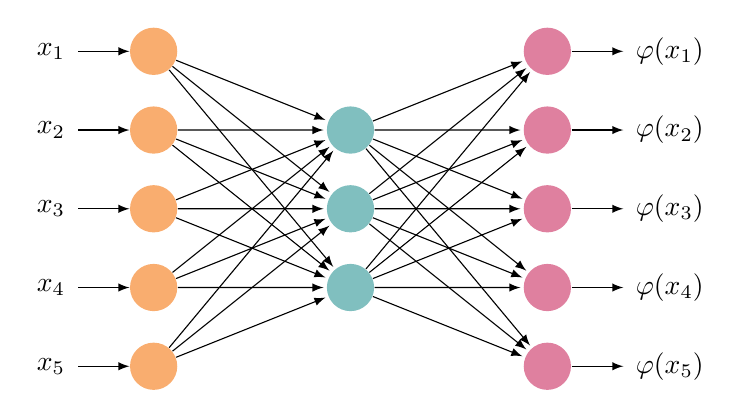
\begin{tikzpicture}
\foreach \i in {1,...,\inputs}
{
	\node[circle,
		minimum size = 6mm,
		fill=Apricot] (Input-\i) at (0,-\i) {};
}

\foreach \i in {1,...,\hiddens}
{
	\node[circle,
		minimum size = 6mm,
		fill=teal!50,
		yshift=(\hiddens-\inputs)*5 mm
	] (Hidden-\i) at (2.5,-\i) {};
}

\foreach \i in {1,...,\outputs}
{
	\node[circle,
		minimum size = 6mm,
		fill=purple!50,
		yshift=(\outputs-\inputs)*5 mm
	] (Output-\i) at (5,-\i) {};
}

\foreach \i in {1,...,\inputs}
{
	\foreach \j in {1,...,\hiddens}
	{
		\draw[-latex, shorten >=1pt] (Input-\i) -- (Hidden-\j);
	}
}

\foreach \i in {1,...,\hiddens}
{
	\foreach \j in {1,...,\outputs}
	{
		\draw[-latex, shorten >=1pt] (Hidden-\i) -- (Output-\j);
	}
}

\foreach \i in {1,...,\inputs}
{
	\draw[latex-, shorten >=1pt] (Input-\i) -- ++(-1,0)
		node[left]{$x_{\i}$};
}

\foreach \i in {1,...,\outputs}
{
	\draw[-latex, shorten >=1pt] (Output-\i) -- ++(1,0)
		node[right]{$\varphi(x_{\i})$};
}

\end{tikzpicture}
